\section{6. Competition}

\subsection*{Competitor Analysis}
\begin{table}[h!]
    \centering
    \renewcommand{\arraystretch}{1.5}
    \begin{tabular}{|>{\bfseries}m{0.2\textwidth}|m{0.25\textwidth}|m{0.25\textwidth}|m{0.25\textwidth}|}
    \hline
    \textbf{Competitor} & \textbf{Strengths} & \textbf{Weaknesses} & \textbf{DynoCharge Edge} \\
    \hline
    Ionity & 350kW chargers, highway dominance & High prices (€0.43/kWh), no rural coverage & 20\% lower pricing, rural focus \\
    \hline
    Shell Recharge & Brand recognition, 50k+ stations & Slow chargers (50kW), no renewables & 3x faster charging, solar integration \\
    \hline
    Tesla & Exclusive network, loyalty & Closed ecosystem, limited compatibility & Open to all EVs, unified app \\
    \hline
    \end{tabular}
    \caption{Competitor Analysis}
\end{table}

\subsection*{Market Share (2024)}
\begin{itemize}
    \item Tesla: 25\%
    \item Shell Recharge: 20\%
    \item Ionity: 15\%
    \item Others: 40\%
\end{itemize}

\subsection{Market Share of Competitors}
\begin{figure}[h!]
    \centering
    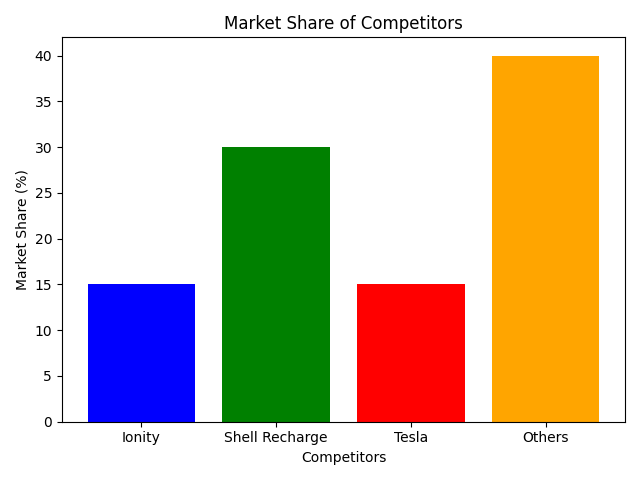
\includegraphics[width=0.8\textwidth]{images/Marketshare.png}
    \caption{Market share of competitors in the EV charging industry.}
    \label{fig:market_share}
\end{figure}
